% -*- TeX-master: "report" -*-

\section{Experiments}

This section presents quantitative data about the ideas presented in previous sections.  This data was collected using the Siemens test suite \cite{257766} as maintained by the Galileo Software-artifact Infrastructure Repository (SIR) \cite{Do05,SAI}.  There are two configurable parameters for the experiments: the rate of sampling and $\effort$ (described in \autoref{sec-metrics}).  Unless specified, the default sampling rate is 1 (i.e., complete data collection) and the default $\effort$ is 5\% (only predicates that are reachable from each other by exploring less than 5\% of the program are considered).  Each Siemens application is available in multiple variants with different bugs: as few as 9 variants of \texttt{schedule2} and as many as 41 variants of \texttt{tcas}.  We report aggregate results by averaging the relevant measures across all variants of each Siemens application.

\subsection{Top Scoring Predicates}

\label{sec-quant}
\begin{figure}
  \centering
  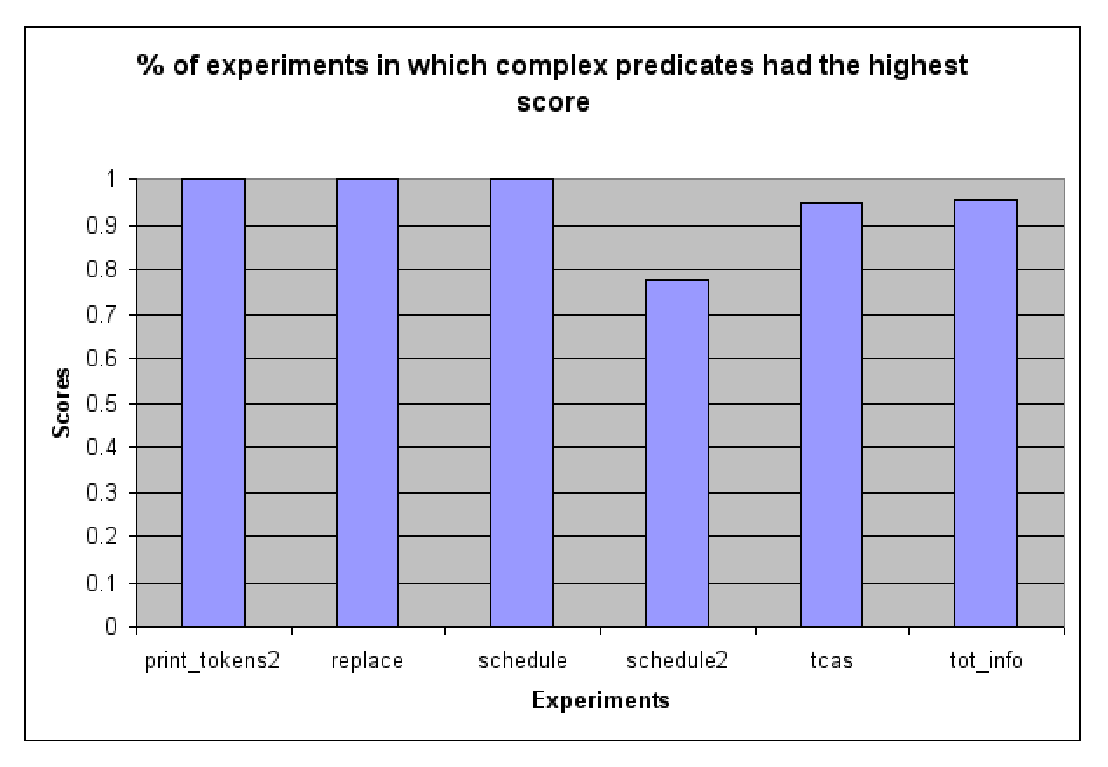
\includegraphics{charts/top-pred}
  \caption{Fraction of buggy application variants having a complex predicate as the top-scoring predictor}
  \label{fig-top-pred}
\end{figure}

\autoref{fig-top-pred} plots the percentage of variants within each program for which a complex predicate had the highest score among all predicates.  The value is 100\% for \texttt{print\_tokens2, replace} and \texttt{schedule} and is close to 100\% for the other programs.  The results shown in \autoref{fig-top-pred} combined with the case studies in \autoref{sec-qual} demonstrates the usefulness of complex predicates.

\subsection{Effectiveness of Pruning}

\begin{figure}
  \centering
  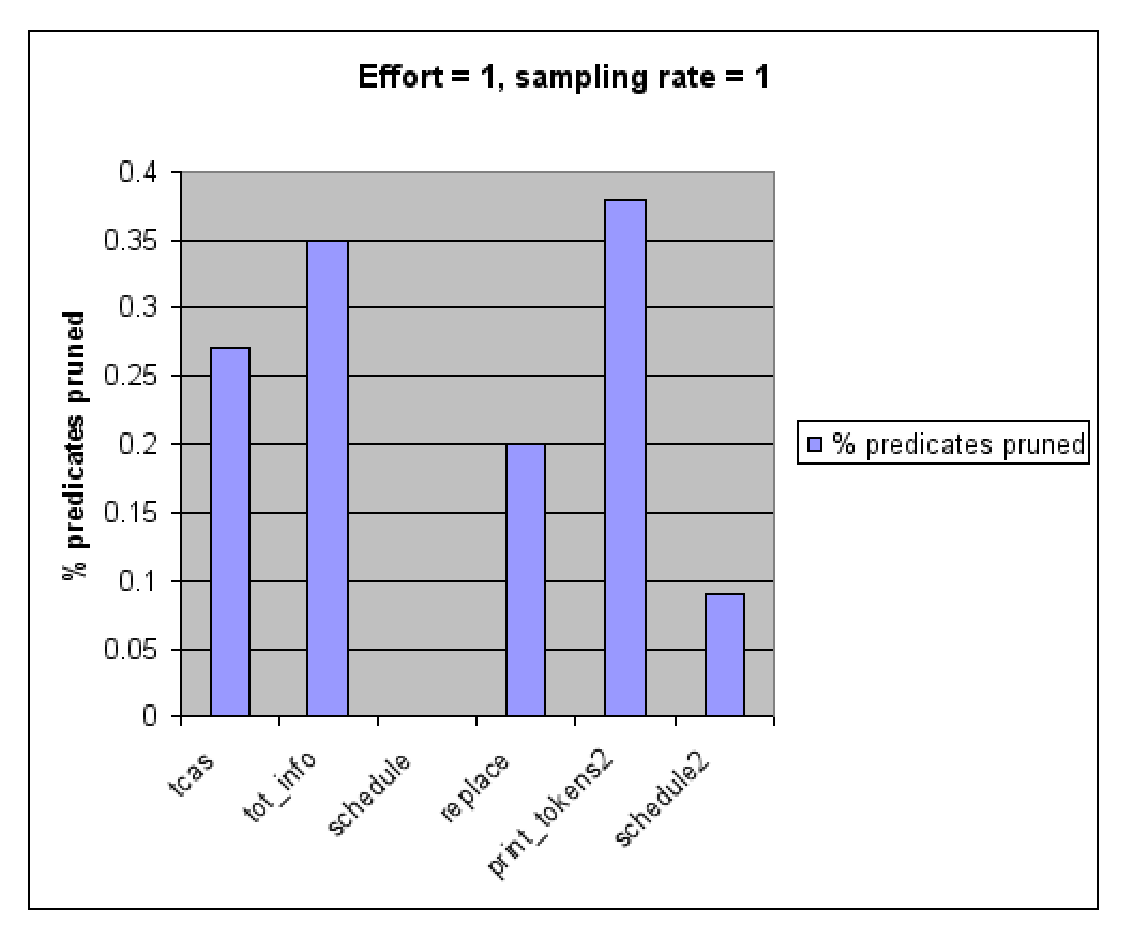
\includegraphics{charts/pruning}
  \caption{Avoiding computing exact scores by pruning complex predicates.  ``Overall'' summarizes the entire Siemens suite.}
  \label{fig-pruning}
\end{figure}

Even when restricted to binary conjunction and disjunction, complex predicates could substantially increase the analysis workload if na\"ively implemented.  \autoref{sec-metrics} suggests heuristics for pruning complex predicates which are unlikely to be useful or understandable to a programmer, while \autoref{sec-pruning} describes how to compute an upper bound on a predicate's score.  \autoref{fig-pruning} shows that these measures are highly effective in practice.  On average, 57\% of candidate complex predicates are discarded because the $\effort$ as defined in \autoref{def-effort} would require traversing more than 5\% of the application code.  A further 14\% of complex predicates are pruned because the upper bounds of their $\Importance$ scores, computed per \autoref{sec-pruning}, are lower than the scores of their constituent simple predicates.  Only 29\% of complex predicates remain.  Thus, exact scores need be computed for less than a third of the initial pool of complex predicates.

\subsection{Effect of Effort}

\begin{figure}
  \centering
  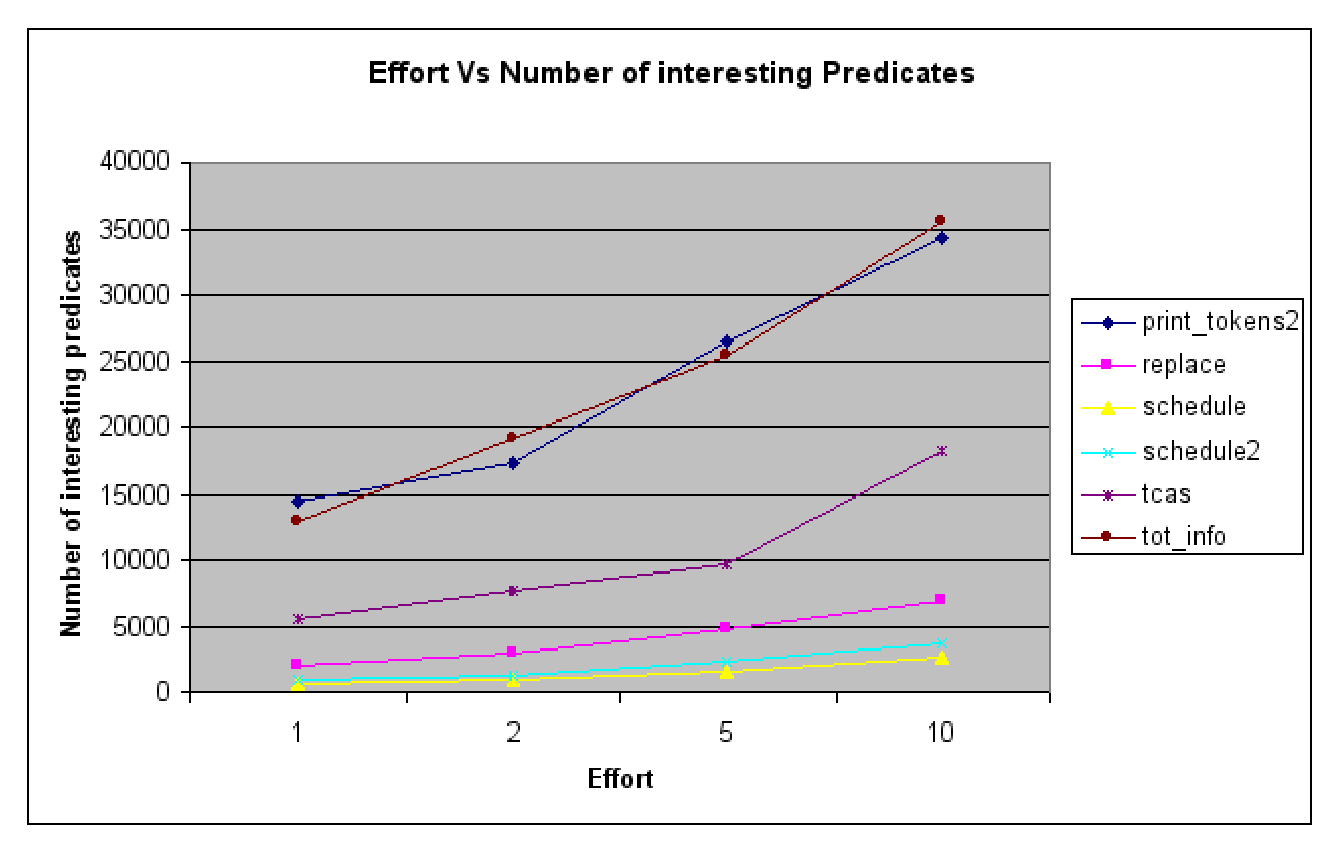
\includegraphics{charts/effort}
  \caption{Variation of number of interesting predicates with $\effort$}
  \label{fig-effort}
\end{figure}

\autoref{fig-effort} has one curve for each program showing how the number of interesting predicates (\autoref{dfn3}) varies at four different values - 1, 2, 5, 10 for $\effort$.  As expected, as $\effort$ increases more predicates are evaluated and so more interesting predicates are found.  This experiment serves as a sanity check for the implementation.

\subsection{Effect of Sampling Rate}
\label{sec-sampling}

\begin{figure*}
  \centering
  $\begin{array}{cc}
    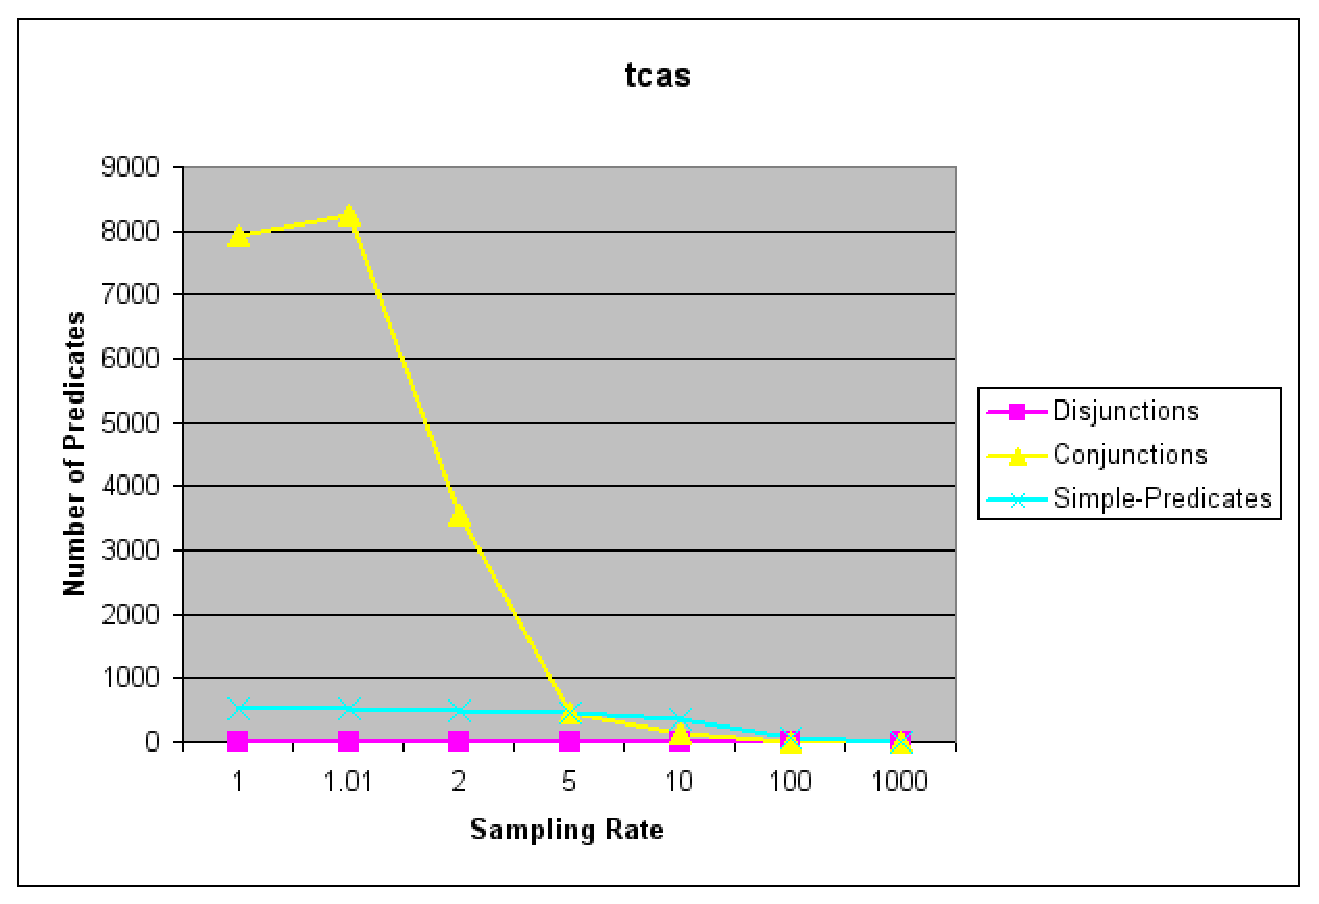
\includegraphics[width=\columnwidth]{charts/tcas} & 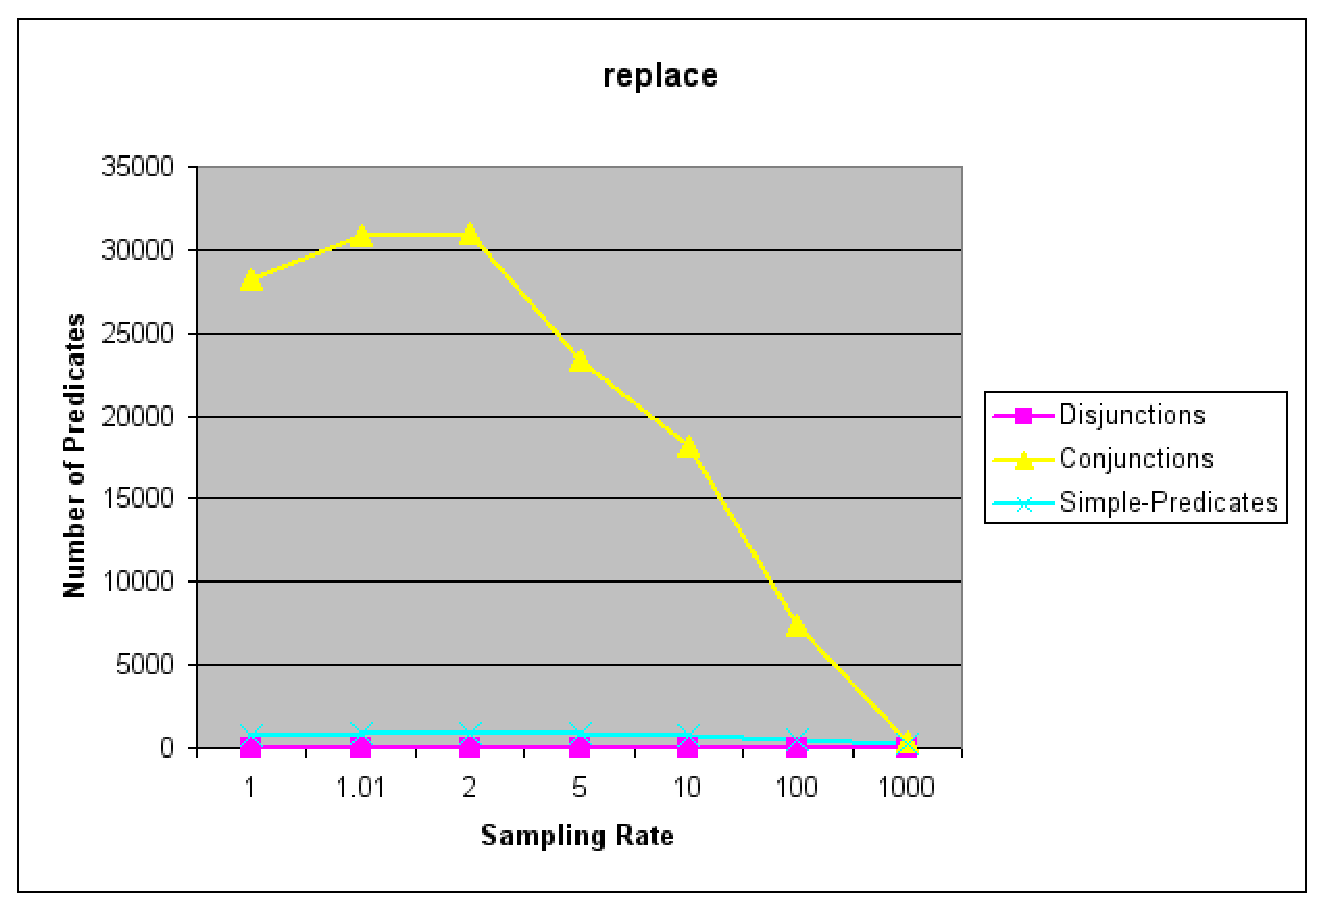
\includegraphics[width=\columnwidth]{charts/replace} \\
    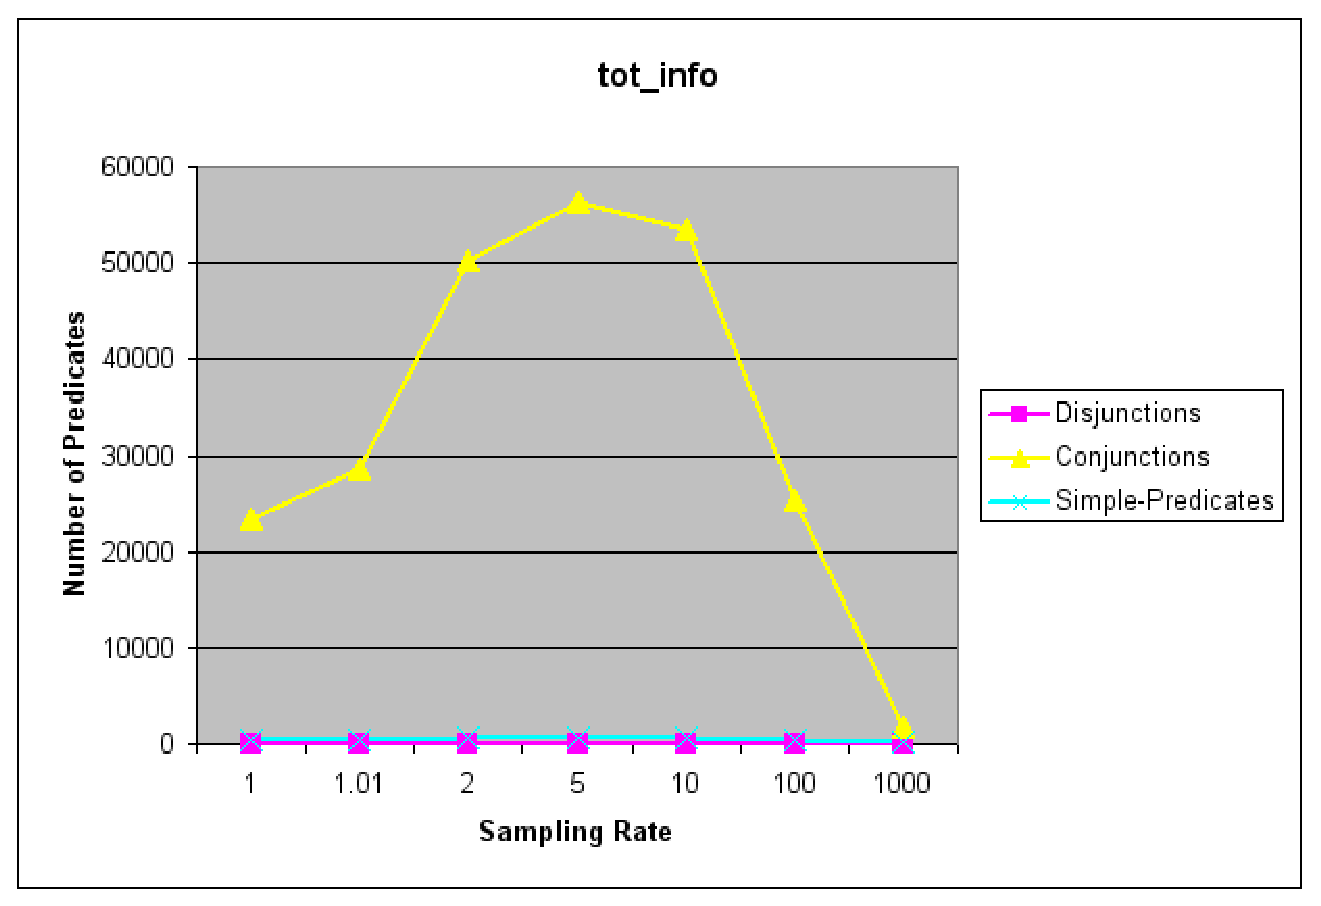
\includegraphics[width=\columnwidth]{charts/tot_info} & 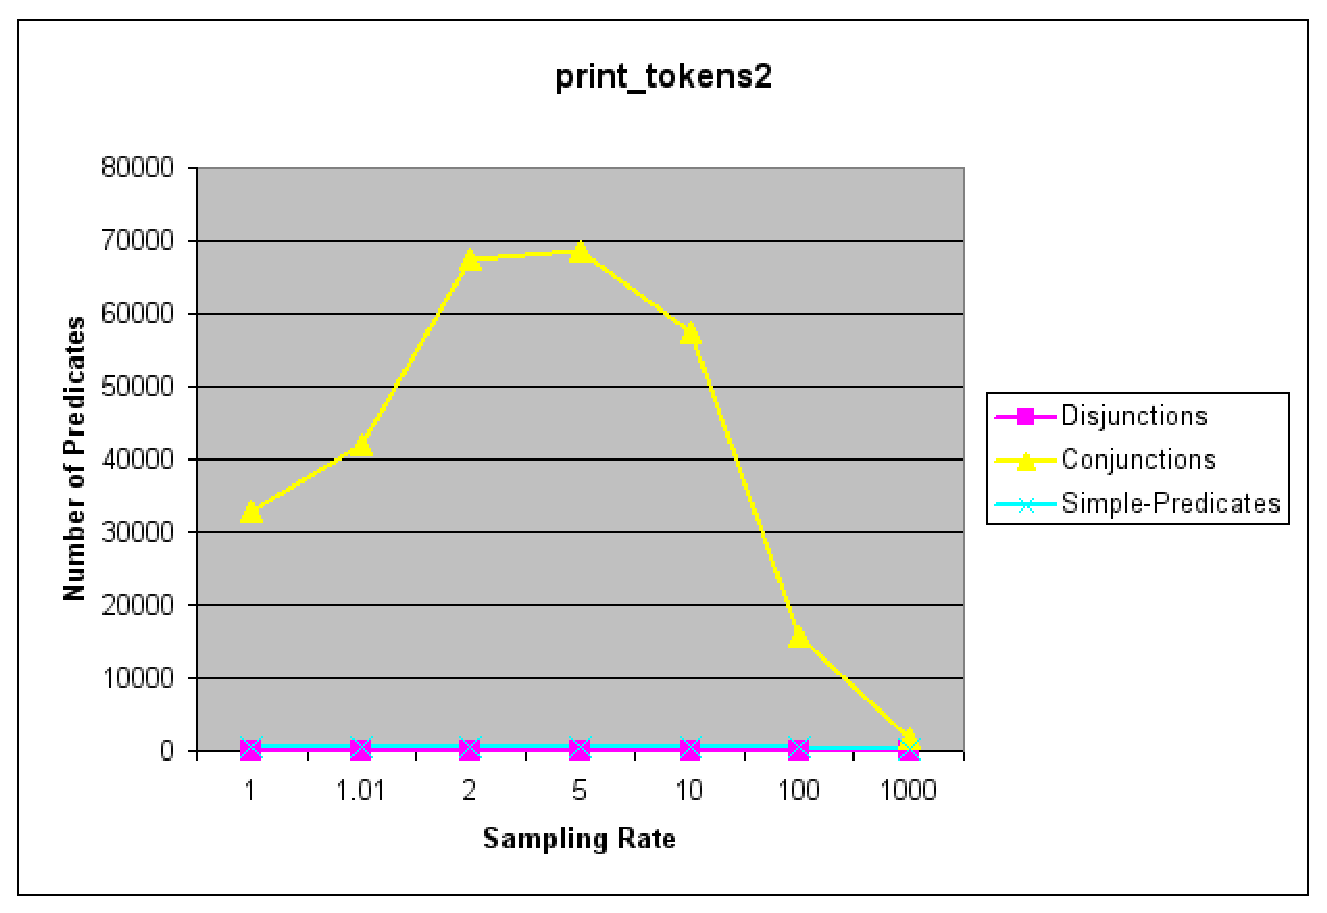
\includegraphics[width=\columnwidth]{charts/print_tokens2} \\
    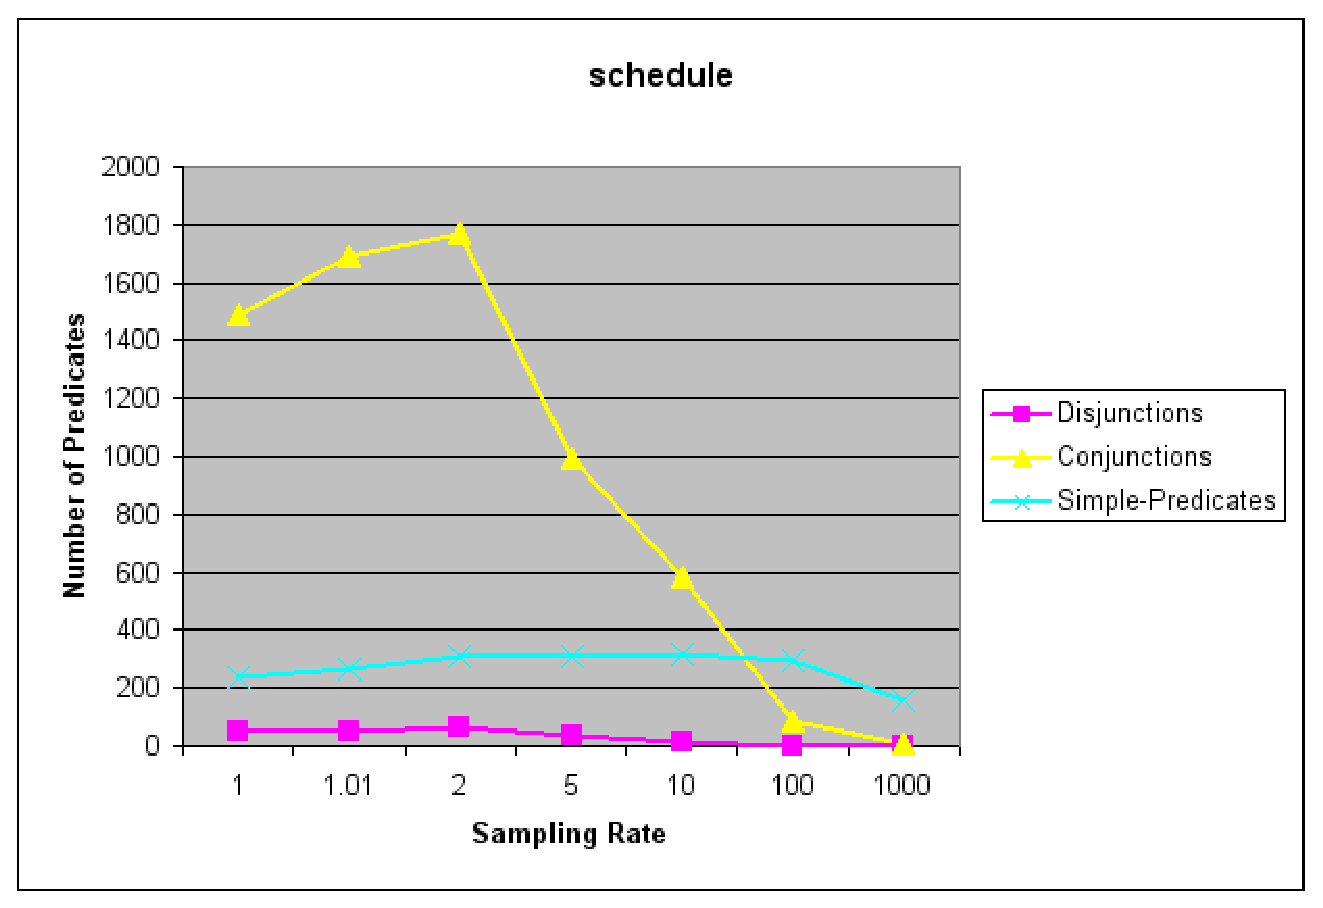
\includegraphics[width=\columnwidth]{charts/schedule} & 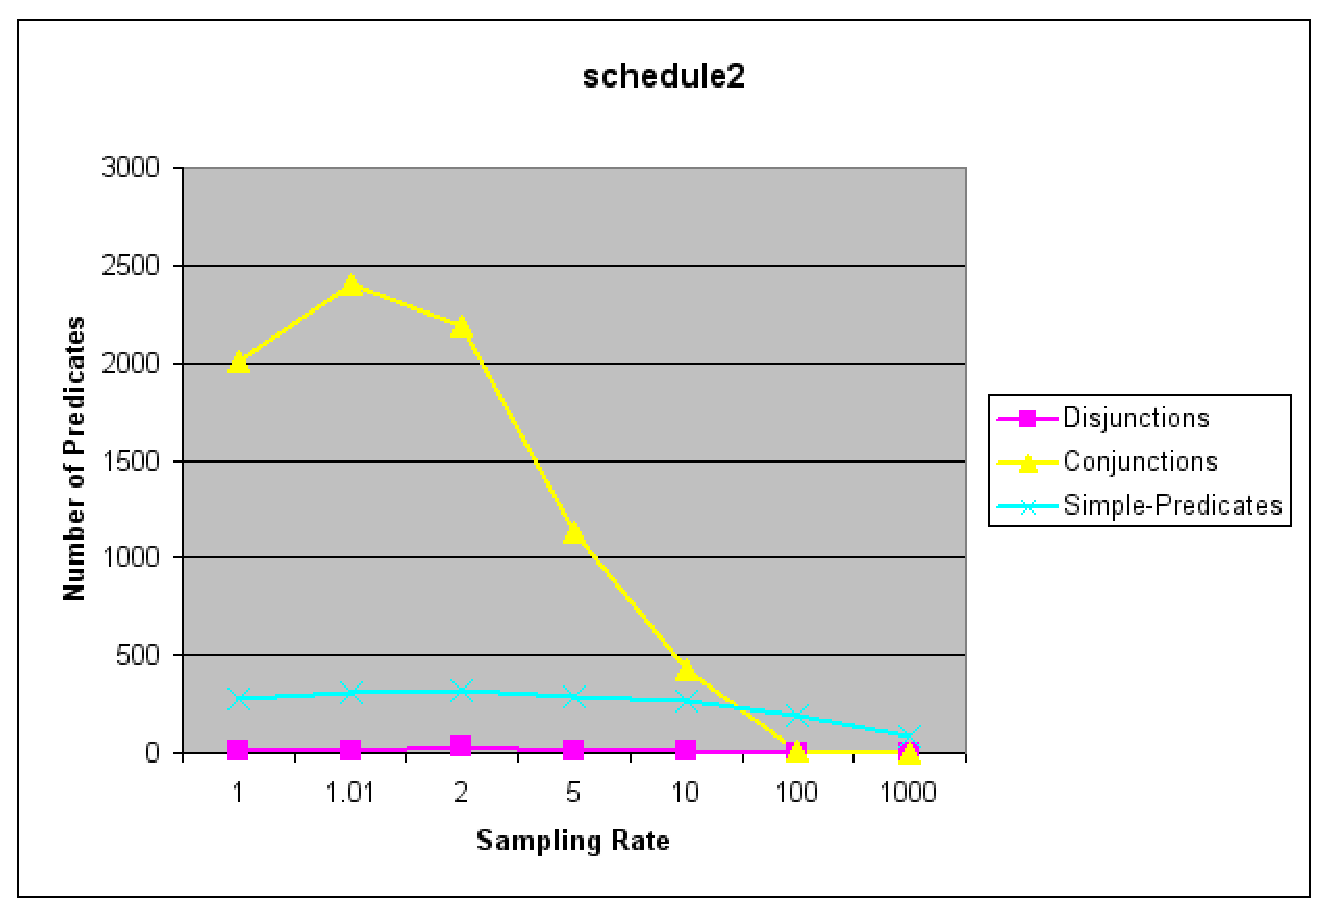
\includegraphics[width=\columnwidth]{charts/schedule2} \\
  \end{array}$
  \caption{Sampling Rate vs. Number of Interesting Predicates}
  \label{fig-sampling}
\end{figure*}

The dependence between sampling rate and the number of interesting predicates (both complex and simple) is plotted in \autoref{fig-sampling}.  \autoref{fig-sampling} has one chart per program with sampling rates in the $x-$axis and the average number of interesting conjunctions, disjunctions and simple predicates in the $y-$axis.  The number of interesting disjunctions is always very low (order of tens) compared to interesting conjunctions.  So the plot for interesting complex predicates closely follows the plot for conjunctions.  At sampling rates lower than \nicefrac{1}{10}, there is a sharp drop in the number of interesting conjunctions.  This is because the chance of observing both components of a conjunction within a single run falls with the square of the sampling rate.  Despite the sharp drop, the number of interesting conjunctions is still comparable to the number of interesting simple predicates even at \nicefrac{1}{1000} sampling.  This shows interesting complex predicates can still be found at sparse but realistic sampling rates.

A puzzling trend in \autoref{fig-sampling} is that the number of interesting conjunctions increases for a brief interval before dropping off.  This trend is consistent across all programs.  This can be due to two reasons:
\begin{enumerate}
\item Consider the $\Increase$ score (\autoref{eqn1}).  Sampling may be reducing the number of \emph{observed} runs in which a conjunction was true without affecting the \emph{true} runs.  This could happen because we do not collect sampled data directly but use scripts to downsample a data set collected with no sampling.  Because of binarization of counts, downsampling of a count from 100 to 99 does not affect the score whereas downsampling from 1 to 0 affects the score.
\item The script that does downsampling uses the standard pseudo random number generator.  Usually for experiments that use such random data, the values are averaged over multiple trials to get a confident estimate of the results.  We weren't able to conduct multiple trials because of time constraints.
\end{enumerate}
